\documentclass[12pt]{report}
\usepackage[a4paper,left=25mm, right=25mm, top=30mm, bottom=30mm]{geometry}
\usepackage[english]{babel}
\usepackage[utf8x]{inputenc}
\usepackage{amsmath}
\usepackage{graphicx}
\usepackage{wrapfig}
\usepackage{microtype}
\usepackage{setspace}
\usepackage{enumitem}


\usepackage[nottoc]{tocbibind}
\usepackage{natbib}
\usepackage[section]{placeins}

\usepackage{graphicx}
\usepackage{lscape}
\usepackage{amssymb}
\usepackage{epstopdf}
\usepackage{algorithm}
\usepackage{algorithmic}
\usepackage{subfig}
\usepackage{float}
\usepackage{wrapfig}
\usepackage{fancyhdr}
\usepackage{natbib}
\captionsetup{margin=10pt,font=small,labelfont=bf}
\usepackage[raggedright]{titlesec}
\usepackage{amsmath}
\usepackage{titlesec}
\usepackage{lipsum}
\usepackage{parskip} 


\renewcommand{\familydefault}{\sfdefault}
\setstretch{1.25}
\graphicspath{ {./images/} }
\bibliographystyle{agsm} %agsm

\titleformat{\chapter}[display]
  {\normalfont\bfseries}{}{0pt}{\huge}
\begin{document}
\begin{titlepage}

   

    \title{ 
\includegraphics[scale=1.7]{utslogo.jpg}\\[1cm]  
    Faculty of Engineering and Information Technology\\[1.0cm] 
    \Large{\textbf{Human Body 3D Scanner (Virtual me)}}\\}
    \author{Esteban Andrade\\ 
    12824583\\
    Supervisor: Dr Teresa Vidal Calleja\\}
    \date{\today}  
     \maketitle
     \cleardoublepage
\end{titlepage}

\addtocontents{toc}{\protect\thispagestyle{empty}}
\tableofcontents
\thispagestyle{empty}
\newpage
\setcounter{page}{1}

\chapter{Engineering Reseach Problem}

\section{Reseach Question}
\textit{\large{"Human Body 3D Scanner: The development of software for 3D data reconstruction of a Human body scanner with multiple sensors" }}

\section{Project Contextualization}
The project is based on creating a Human Body 3D scanner.
It will have two specific streams that include the development of  the mechatronic design of a 3D scanner for a human and the software development for 3D data reconstruction. 
This proposal is based on developing the software for 3D data modelling and reconstruction of the Scanned data.\\[10pt]
Similarly, with the 3D reconstructed model of the human has the aim to be utilised to test different fashion clothing items. This has the intent to adjust the sizing of the clothes fittings based on the Scanned data. The clothing models will adjust automatically depending on the dimensions of the data of the scanned model. 
   
\section{Problem Definition}
Being able to obtain data from multiple sensors and model objects has is very crucial for many industries.
Nevertheless, there is a lack of precise and accurate options in the market that could create 3D models of Humans with respective sensor data. Similarly there are no current industry application that maximise the potential use of the Human body 3D models.
Therefore, this project is aimed at creating a solution and develop the software for 3D data reconstruction of the scanned human. This model will be utilised to try different fashion items and adapt the size fittings accordingly. \\[10pt]
The project will have different stages that range from testing different sensors for data acquision, testing different data stitching frameworks to the deployment of the software in the 3D scanner mechatronic device. 
\enlargethispage{\baselineskip}

\section{Background}
The human society has the world comprenhension of the surrouding world through visual perception. This principle allows to differenciate distintive kinds of shapes, objects,colours, textures and the spatial pose of the surroudings.
Based on this information, it is possible to analyse the number of objects in a determined location, object type, object size, object pose in different coordinate frames. 
Thus, it impacts how as a society we interactuate with objects ot scenes. As a result it is essential to imitate this perception in order to acquire real world data in different formats that include:
\begin{itemize}[]
    \item RGB images
     \item Depth images
     \item 3D point clouds 
     \item Multispectral images
     \item Laser readings
\end{itemize}
All these acquire data can be obtained from a wide variety of comercial or industrial sensors. With this data it will be possible to use computer processing techniques in order to model the object or scene \citep*{murcia_monroy_mora_2018}.

\section{Applications}
In the recents years the use of 3D body scanners has gain importance in several industries. Within the fashion industry it can aid clothes manufactures to obtain accurate body measurement data of body dimensions.
As mentioned by \citet*{sturm_bylow_kahl_cremers_2013}, this new technological approach has the potential to alterate the future of the fashion and clothing manufacturing industry.

With the raise of innovatoin of 3D image reconstruction, the interest from to gather precise measurements of the human has raised. Due to the fact, that in the clothing industry
is extremedely important to create better fittings for different shapes of human bodies. 
Furthermore, virtual try-on solutions has gain popularity in physical and online retail stores \Citep*{spahiu_shehi_piperi_2014}.

On the other side 3D scanners have gain in particupation in the medical industry. These systems are described as "non-invasive and low cost" , thus making it appealing for epidemiological surveys and clinical uses. \Citep*{treleaven_wells_2007}
The geometrical measurements could be associated with shape, size, volume and surface area of the body parts. It could aid to be a sustainable approach to screen children and patients with obesity, deformities or specific anatomic defects. 
Therefore, it will ease the diagnose process and allow to treat and monitor medical conditions holisticly and improve the life quality of patients with non-invasive tests.
The table below illustrates the use of 3D scanner in the medical field with the purpose to identify and monitor various medical conditions. 
Frpm which the diagnose, treatment and monitor procedures willd differ based on the acquired data.
\begin{table}[ht]
    \centering
    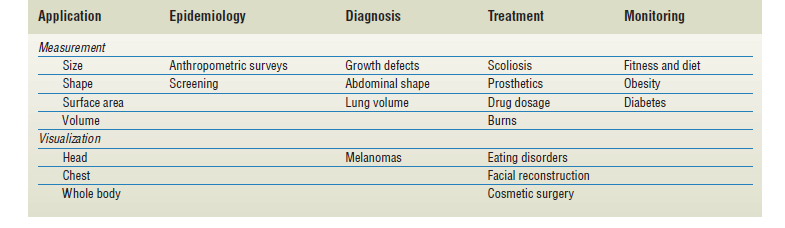
\includegraphics[width=15cm]{table1.png}
    \caption{3D Scanning Applications \cite[]{treleaven_wells_2007}.}
\end{table}

\begin{figure}[h]
  \begin{center}
  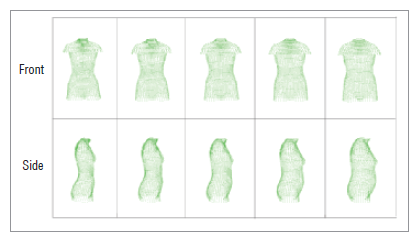
\includegraphics[width=0.5\textwidth]{bodyMedicine.png}
  \caption{Front, Side results of 3D Scanning \cite[]{treleaven_wells_2007}.}
  \label{bodymed}
\end{center}
\end{figure}


\chapter{Related Works}
Being able to scan different objects and subjects has been challeging task for researchers. Getting an accurate spatial location of the objects is crucial for this  type of application.
The use of 3D point clouds has facilitated this process as it allows to obtain the following parameters:
\begin{itemize}[]
  \itemsep0em 
  \item Depth
  \item Intensity
  \item Pulse width
  \item Light echo
\end{itemize}
This information can be obtain with different kind of sensors. There is a wide variety of off the shelf sensors that can procide 3D point clouds. 
These sensors could either be stereo or multiview vision cameras, lasers, time-of-flight sensors (\textit{TOF}) and structured light sensors as stated by \Citet*{murcia_monroy_mora_2018}.

Many Scanning devices will use single or multiple of the above-mentioned sensors in order to acquire data. Once the data is obtained, it essential to have a framework for 3D data modelling and reconstruction.
The principle behind 3D data recontruction is obtained with data fision from RGB-D sensors. This kind of sensors provide 3 channels images RGB (red,green, blue) and the depth images are mapped to each pixel. Based on this data 3D point clouds could be generated for data recontruction.
One of the most common frameworks is known as \textbf{Dynamic Fusion} which is referenced to \textit{"reconstruction and tracking of Non-rigid Scenes in real time"} \Citep*{newcombe_fox_seitz_2015}.
Another recent powerful 3D Data recontruction framwork is \textbf{SurfelWarp} which is defined as \textit{"Efficient Non-Volumetic Single View Dynamic Reconstruction"} \Citep*{SurfelWarp}.


\section{Dynamic Fusion}
Dynamic fusion is the mesh and fusion of three techniques used for 3D scanning and reconstruction.  These techniques are:

\begin{description}[style=nextline]
    \item[Kinect Fusion] Used for real-time Dense surface Mapping and tracking. This technique is designed for static scenes and objects only with a moving camera
    \item[DART (Dense Articulated Real Time Tracking)] This technology is focused on Real Time template tracking.
    \item[Animation Cartography] 3D reconstruction technique used for intrinsic Reconstruction of shapes and motions. 
\end{description}

\begin{wrapfigure}{r}{0.5\textwidth} %this figure will be at the right
    \centering
    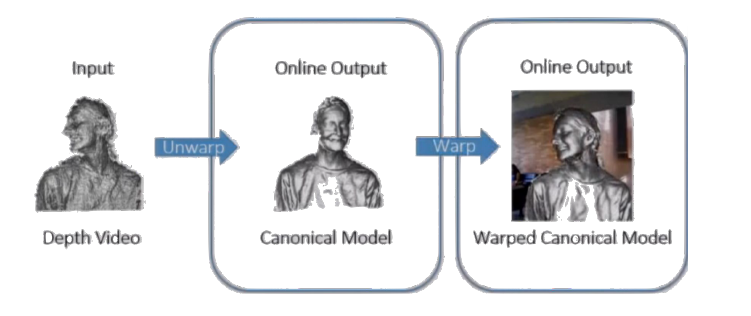
\includegraphics[width=0.5\textwidth]{IMG_0073.png}
    \caption{Transformation Between Depth Video to Warped canonical Model. \cite[]{newcombe_fox_seitz_2015}}
\end{wrapfigure}
The principal focus of Dynamic fusion, 3D reconstruction technique, is that once the data is gathered, it will solve for a volumetric flow field. 
This will transform the state of the scene at each time instant into a fixed canonical frame as developed by Newcombe, Fox and Seitz (2015). \\[10pt]
The canonical frame is known as the first frame that is captured from the non-rigid object that has been tracked and scanned. The canonical model is the shape of the object that is defined in the canonical frame. 
Thus, the canonical model will be used as reference for other frames and there will be cumulative refinement on this model and frames, as more scans and  measurements are taken.
With the new refinements each point in the canonical frame, which will be point cloud will be transformed to its new location in the real time frame.\\[10pt]
The volumetric flow field will be estimated with the help of the warp field parameters using the live depth video from the sensors. 
The state of the wrap field W\textsubscript{t} is defined as a function of time and defined by the values of a set of n deformation nodes, which are points in the actual image
\[N_{warp}^t=\{dg_v,dg_w,dg_{se3}\}t\]
\begin{itemize}[label =]
    \item $dg_{v}$: Used for real-time Dense surface Mapping and tracking. This technique is designed for static scenes and objects only with a moving camera
    \item $dg_{se3}$: This technology is focused on Real Time template tracking.
    \item $dg_{w}$: 3D reconstruction technique used for intrinsic Reconstruction of shapes and motions. 
\end{itemize}

The current level set of point clouds will be stored as a polygon mesh, with normal pairs points in the canonical frame, that later will be used for surface reconstruction.   
Slavcheva, Baust and Ilic, (2018)  mention that once the warp field parameters are obtained from the data, the surface reconstruction can be modelled using Marching Cubes, followed by the rasterization rendering pipeline of the Acquired Point cloud values.\\
\begin{wrapfigure}{l}{0.5\textwidth} %this figure will be at the right
    \centering
    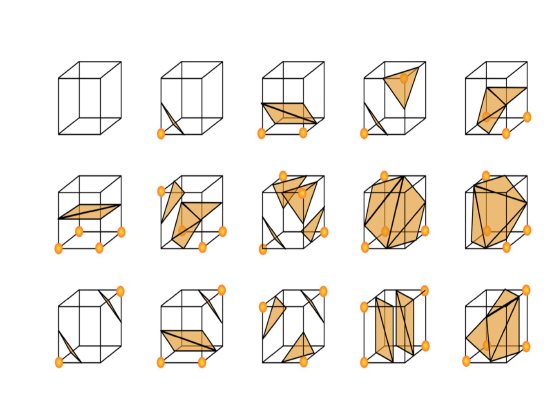
\includegraphics[width=0.5\textwidth]{shapes.png}
    \caption{Triangulated patterns \cite[]{fang_zhao_wen_zhang_2018}}
\end{wrapfigure}
These 15 patterns from the image 3 represent the Triangulated cubes for the 15 basic patterns used in Marching Cubes for the method of surface reconstruction. These patterns can reconstruct all the 256 possible solutions using complementary and rotational symmetry (Fang, Zhao, Wen and Zhang, 2018).
\begin{figure}{l} %this figure will be at the right
    \centering
    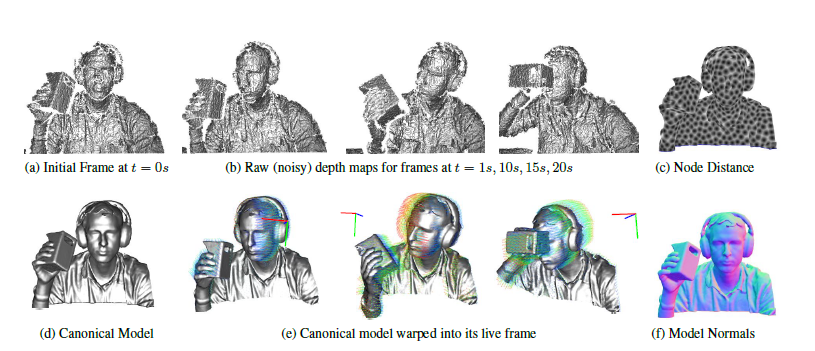
\includegraphics[width=0.7\textwidth]{dynamicfusion2.png}
    \caption{Dynamic Fusion methodology \cite[]{newcombe_fox_seitz_2015}}
\end{figure}
Once the canonical model, and frame and warp field parameters are obtained from the initial data frame and raw depth maps, the nodes will be created. Then the canonical frame warp parameters will be estimated. Once the canonical model is created it will be warped to its live frame with help of the warp parameters and then the model normalised and is created. \\
\enlargethispage{\baselineskip}











 \nocite{*}   % all not cited bib entrys are shown in bibliography ...
\bibliography{resources}
\end{document}
